\subsection{Getting doping from resistance}
In many cases the supplier will only provide the resistance per length specification for their substrate and won't give you the dopant concentration numbers.
In this case you will have to find these numbers out yourself by converting it from the numbers they've provided.

\begin{figure}[H]
	\centering
	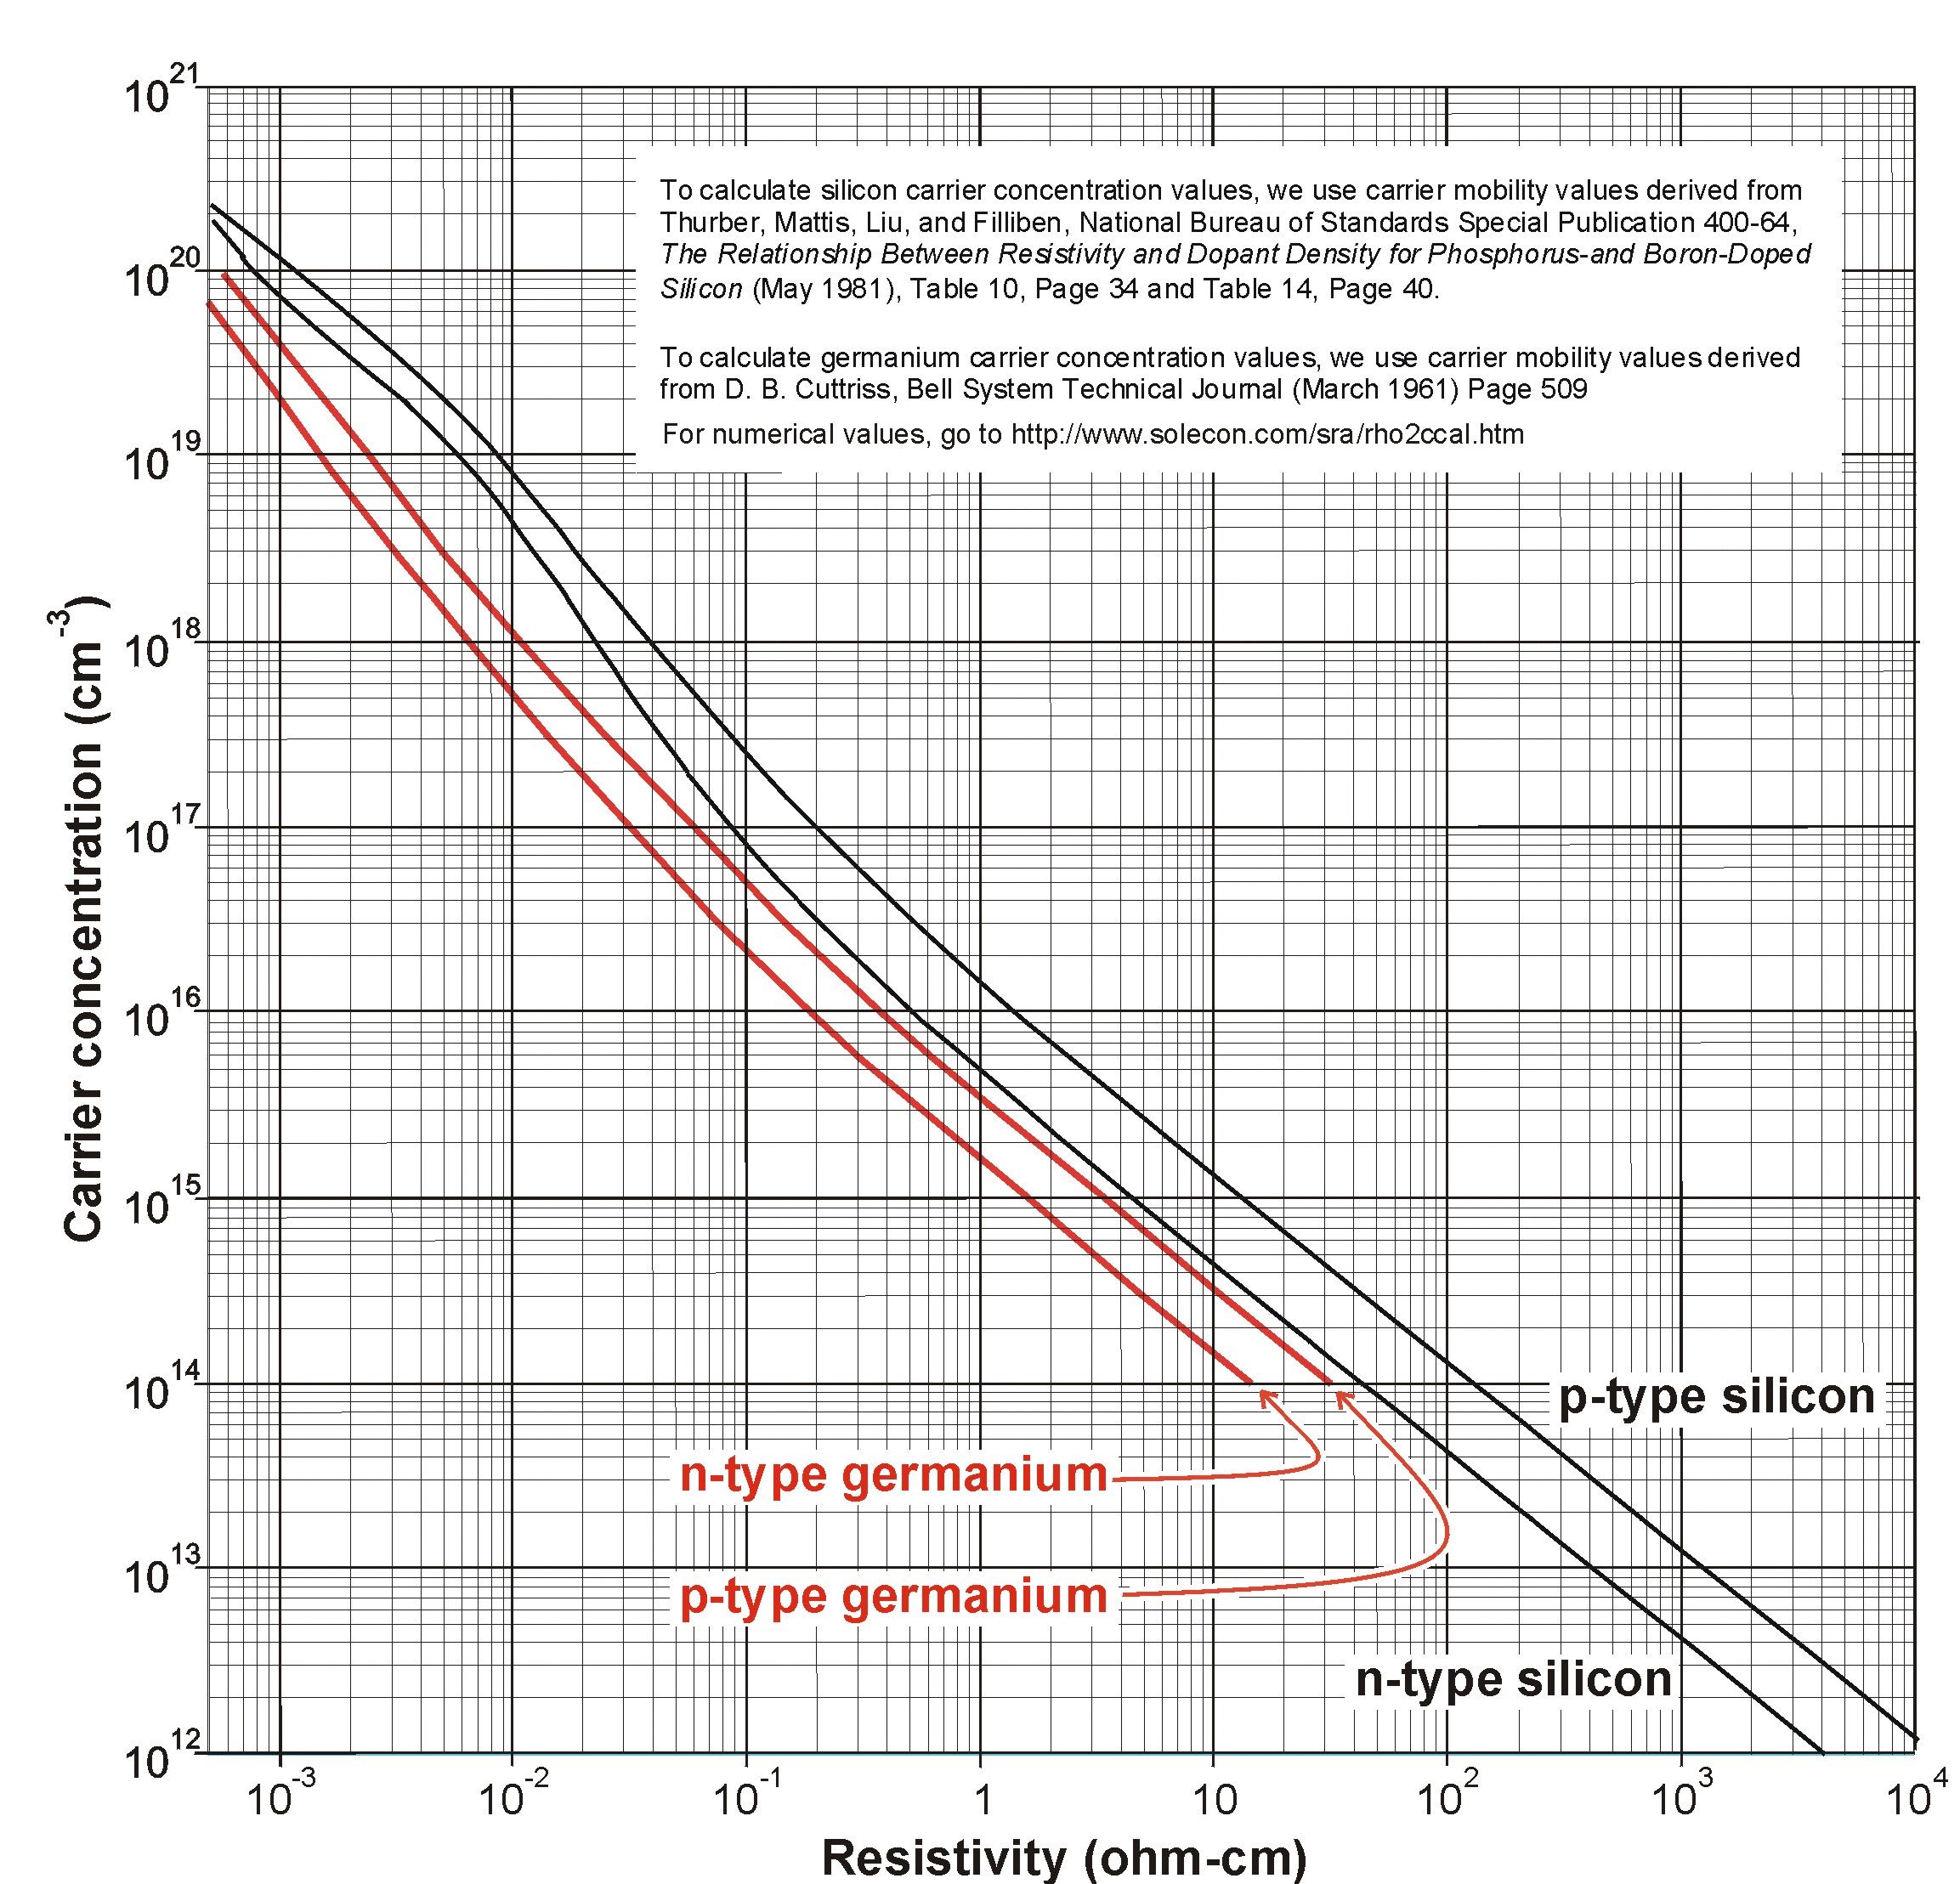
\includegraphics[width=0.5\textwidth]{resistance_doping.png}
	\caption{R-L-dopant relation}
	\label{r_l_nd_relation}
\end{figure}

You can either use the graphics from \autoref{r_l_nd_relation} and determine the dopant concentration graphically, which is very very imprecise or use a online tool like the one from Solecon\footnote{\url{http://www.solecon.com/sra/rho2ccal.htm}}

Germanium is being included in this graphics just in case someone is going to fork this process based on Germanium substrate.